\documentclass[12pt]{article}

% ── Packages ─────────────────────────────────────────────────────────────────
\usepackage[margin=1in]{geometry}
\usepackage{booktabs}
\usepackage{graphicx}
\usepackage{amsmath}
\usepackage{hyperref}
\usepackage{setspace}
\usepackage[T1]{fontenc}
\usepackage{lmodern}
\usepackage{natbib}

\doublespacing

% ── Load auto-generated numbers ─────────────────────────────────────────────
% Auto-generated by results.qmd. Do not edit by hand.

\newcommand{\NTotal}{182}

\newcommand{\NSolo}{94}

\newcommand{\NAI}{88}

\newcommand{\NProlific}{15}

\newcommand{\NConnect}{167}

\newcommand{\NFlagged}{4}

\newcommand{\NMissingSurvey}{29}

\newcommand{\PctMissingSurvey}{16\%}

\newcommand{\AIUsesMean}{2.1}

\newcommand{\AIUsesSD}{2.5}

\newcommand{\MissChiSq}{1.04}

\newcommand{\MissChiP}{$= .307$}

\newcommand{\EloMeanSolo}{1488.22}

\newcommand{\EloMeanAI}{1517.9}

\newcommand{\EloSDSolo}{91.55}

\newcommand{\EloSDAI}{78.78}

\newcommand{\EloNSolo}{94}

\newcommand{\EloNAI}{88}

\newcommand{\EloT}{2.35}

\newcommand{\EloDF}{179}

\newcommand{\EloP}{$= .020$}

\newcommand{\EloD}{0.35}

\newcommand{\PretrainedMeanSolo}{47.39}

\newcommand{\PretrainedMeanAI}{52.82}

\newcommand{\PretrainedSDSolo}{22.57}

\newcommand{\PretrainedSDAI}{20.84}

\newcommand{\PretrainedNSolo}{76}

\newcommand{\PretrainedNAI}{78}

\newcommand{\PretrainedT}{1.55}

\newcommand{\PretrainedDF}{15}

\newcommand{\PretrainedP}{$= .123$}

\newcommand{\PretrainedD}{0.25}

\newcommand{\LLMHumorMeanSolo}{6.32}

\newcommand{\LLMHumorMeanAI}{6.44}

\newcommand{\LLMHumorSDSolo}{0.73}

\newcommand{\LLMHumorSDAI}{0.73}

\newcommand{\LLMHumorNSolo}{76}

\newcommand{\LLMHumorNAI}{78}

\newcommand{\LLMHumorT}{1.02}

\newcommand{\LLMHumorDF}{152}

\newcommand{\LLMHumorP}{$= .311$}

\newcommand{\LLMHumorD}{0.16}

\newcommand{\LLMCleverMeanSolo}{6.96}

\newcommand{\LLMCleverMeanAI}{7.28}

\newcommand{\LLMCleverSDSolo}{0.97}

\newcommand{\LLMCleverSDAI}{0.8}

\newcommand{\LLMCleverNSolo}{76}

\newcommand{\LLMCleverNAI}{78}

\newcommand{\LLMCleverT}{2.23}

\newcommand{\LLMCleverDF}{145}

\newcommand{\LLMCleverP}{$= .027$}

\newcommand{\LLMCleverD}{0.36}

\newcommand{\LLMFitMeanSolo}{8.38}

\newcommand{\LLMFitMeanAI}{8.49}

\newcommand{\LLMFitSDSolo}{0.67}

\newcommand{\LLMFitSDAI}{0.68}

\newcommand{\LLMFitNSolo}{76}

\newcommand{\LLMFitNAI}{78}

\newcommand{\LLMFitT}{0.97}

\newcommand{\LLMFitDF}{152}

\newcommand{\LLMFitP}{$= .334$}

\newcommand{\LLMFitD}{0.16}

\newcommand{\LLMOverallMeanSolo}{7.14}

\newcommand{\LLMOverallMeanAI}{7.38}

\newcommand{\LLMOverallSDSolo}{0.78}

\newcommand{\LLMOverallSDAI}{0.72}

\newcommand{\LLMOverallNSolo}{76}

\newcommand{\LLMOverallNAI}{78}

\newcommand{\LLMOverallT}{1.98}

\newcommand{\LLMOverallDF}{151}

\newcommand{\LLMOverallP}{$= .050$}

\newcommand{\LLMOverallD}{0.32}

\newcommand{\KeystrokesMeanSolo}{87.4}

\newcommand{\KeystrokesMeanAI}{66.92}

\newcommand{\KeystrokesSDSolo}{103.61}

\newcommand{\KeystrokesSDAI}{88.77}

\newcommand{\KeystrokesNSolo}{94}

\newcommand{\KeystrokesNAI}{88}

\newcommand{\KeystrokesT}{1.44}

\newcommand{\KeystrokesDF}{179}

\newcommand{\KeystrokesP}{$= .153$}

\newcommand{\KeystrokesD}{0.21}

\newcommand{\DurationMeanSolo}{117.1}

\newcommand{\DurationMeanAI}{107.99}

\newcommand{\DurationSDSolo}{100.27}

\newcommand{\DurationSDAI}{122.28}

\newcommand{\DurationNSolo}{94}

\newcommand{\DurationNAI}{88}

\newcommand{\DurationT}{0.55}

\newcommand{\DurationDF}{169}

\newcommand{\DurationP}{$= .585$}

\newcommand{\DurationD}{0.08}

\newcommand{\ProcAgencyMeanSolo}{8.86}

\newcommand{\ProcAgencyMeanAI}{6.4}

\newcommand{\ProcAgencySDSolo}{1.78}

\newcommand{\ProcAgencySDAI}{3.91}

\newcommand{\ProcAgencyNSolo}{76}

\newcommand{\ProcAgencyNAI}{77}

\newcommand{\ProcAgencyT}{5.03}

\newcommand{\ProcAgencyDF}{107}

\newcommand{\ProcAgencyP}{$< .001$}

\newcommand{\ProcAgencyD}{0.81}

\newcommand{\OutAgencyMeanSolo}{5.46}

\newcommand{\OutAgencyMeanAI}{5.68}

\newcommand{\OutAgencySDSolo}{2.43}

\newcommand{\OutAgencySDAI}{2.94}

\newcommand{\OutAgencyNSolo}{75}

\newcommand{\OutAgencyNAI}{76}

\newcommand{\OutAgencyT}{0.52}

\newcommand{\OutAgencyDF}{145}

\newcommand{\OutAgencyP}{$= .606$}

\newcommand{\OutAgencyD}{0.08}

\newcommand{\MeaningMeanSolo}{5.32}

\newcommand{\MeaningMeanAI}{4.58}

\newcommand{\MeaningSDSolo}{2.7}

\newcommand{\MeaningSDAI}{3.21}

\newcommand{\MeaningNSolo}{75}

\newcommand{\MeaningNAI}{76}

\newcommand{\MeaningT}{1.52}

\newcommand{\MeaningDF}{145}

\newcommand{\MeaningP}{$= .131$}

\newcommand{\MeaningD}{0.25}

\newcommand{\IdentityMeanSolo}{6.36}

\newcommand{\IdentityMeanAI}{6.13}

\newcommand{\IdentitySDSolo}{2.04}

\newcommand{\IdentitySDAI}{2.44}

\newcommand{\IdentityNSolo}{76}

\newcommand{\IdentityNAI}{77}

\newcommand{\IdentityT}{0.62}

\newcommand{\IdentityDF}{147}

\newcommand{\IdentityP}{$= .536$}

\newcommand{\IdentityD}{0.1}



% ── Title ────────────────────────────────────────────────────────────────────
\title{AI Improves Creative Output but Undermines Process Ownership}
\author{Benjamin Lira Luttges}
\date{}

\begin{document}
\maketitle

% ══════════════════════════════════════════════════════════════════════════════
\section{Methods}
% ══════════════════════════════════════════════════════════════════════════════

\subsection{Participants}

We randomly assigned \NTotal{} participants to write a caption for a \textit{New Yorker}-style cartoon either alone (solo; $n$ = \NSolo) or with access to an AI writing tool (AI; $n$ = \NAI). We recruited \NProlific{} participants from Prolific and \NConnect{} from CloudResearch Connect.

\begin{table}[t]
  \centering
  \caption{Sample by condition and recruitment platform.}
  \label{tab:sample}
  % Auto-generated. Do not edit by hand.
\begin{tabular}{lrrr}
\toprule
Condition & Prolific & Connect & Total \\
\midrule
solo & 9 & 85 & 94 \\
ai & 6 & 82 & 88 \\
\midrule
Total & 15 & 167 & 182 \\
\bottomrule
\end{tabular}

\end{table}

All participants passed the honeypot bot check. Automated moderation flagged \NFlagged{} captions, which we retained (excluding them does not change results). \NMissingSurvey{} participants (\PctMissingSurvey) completed the caption task but not the post-task survey; this missingness did not differ by condition ($\chi^2(1)$ = \MissChiSq, $p$ \MissChiP).

\subsection{Procedure}

Each participant viewed a cartoon and wrote the funniest caption they could. Solo participants wrote unaided. AI participants could request AI-generated caption ideas, which they did an average of \AIUsesMean{} times ($SD$ = \AIUsesSD).

After submitting their caption, participants rated their experience on four sets of 0--10 scales: process agency (3 items: ``I felt like I was producing the work,'' ``I felt responsible for the output,'' ``I felt involved in the process''), outcome agency (3 items: ``How capably/effectively/powerfully did you produce a funny caption?''), meaning (3 items: fulfilling, meaningful, mattered), and humor identity (3 items: funny, importance, reflects).

\subsection{Measures}

Three independent methods assessed caption quality: (1) Elo ratings from pairwise votes by other participants, (2) a pretrained humor model (0--100), and (3) LLM judge ratings on humor, cleverness, fit, and overall quality (each 1--10).

Task behavior measures included total keystrokes, task duration (seconds), and number of AI uses.

We computed survey composites as the mean of each scale's items. All four composites showed acceptable internal consistency.

% ══════════════════════════════════════════════════════════════════════════════
\section{Results}
% ══════════════════════════════════════════════════════════════════════════════

Table~\ref{tab:condition} reports condition differences across all dependent variables.

\begin{table}[t]
  \centering
  \caption{Condition differences (solo vs.\ AI). Effect sizes are Cohen's $d$; positive $d$ indicates solo scored higher.}
  \label{tab:condition}
  % Auto-generated. Do not edit by hand.
\begin{tabular}{lrrrrrr}
\toprule
 & \multicolumn{1}{c}{$M_{\text{Solo}}$} & \multicolumn{1}{c}{$M_{\text{AI}}$} & \multicolumn{1}{c}{$\Delta$} & \multicolumn{1}{c}{$d$} & \multicolumn{1}{c}{$t$} & \multicolumn{1}{c}{$p$} \\
\midrule
\multicolumn{7}{l}{\textit{Caption Quality}} \\
Elo rating & 1488.22 & 1517.90 & -29.67 & 0.35 & 2.35 & .020* \\
Pretrained score & 47.39 & 52.82 & -5.43 & 0.25 & 1.55 & .123 \\
LLM: Humor & 6.32 & 6.44 & -0.12 & 0.16 & 1.02 & .311 \\
LLM: Cleverness & 6.96 & 7.28 & -0.32 & 0.36 & 2.23 & .027* \\
LLM: Fit & 8.38 & 8.49 & -0.11 & 0.16 & 0.97 & .334 \\
LLM: Overall & 7.14 & 7.38 & -0.24 & 0.32 & 1.98 & .050* \\
\addlinespace
\multicolumn{7}{l}{\textit{Task Behavior}} \\
Keystrokes & 87.40 & 66.92 & 20.48 & 0.21 & 1.44 & .153 \\
Task duration (s) & 117.10 & 107.99 & 9.11 & 0.08 & 0.55 & .585 \\
\addlinespace
\multicolumn{7}{l}{\textit{Survey Composites}} \\
Process agency & 8.86 & 6.40 & 2.47 & 0.81 & 5.03 & $<$.001*** \\
Outcome agency & 5.46 & 5.68 & -0.23 & 0.08 & 0.52 & .606 \\
Meaning & 5.32 & 4.58 & 0.73 & 0.25 & 1.52 & .131 \\
Identity & 6.36 & 6.13 & 0.23 & 0.10 & 0.62 & .536 \\
\bottomrule
\multicolumn{7}{l}{\footnotesize $\dag$ $p < .10$, * $p < .05$, ** $p < .01$, *** $p < .001$. Positive $d$ = solo higher.} \\
\end{tabular}

\end{table}

\subsection{AI participants wrote funnier captions}

AI-assisted captions earned higher Elo ratings from peer voting ($M_{\text{AI}}$ = \EloMeanAI{} vs.\ $M_{\text{Solo}}$ = \EloMeanSolo; $t$(\EloDF) = \EloT, $p$ \EloP, $d$ = \EloD) and higher cleverness ratings from LLM judges ($t$(\LLMCleverDF) = \LLMCleverT, $p$ \LLMCleverP, $d$ = \LLMCleverD). Humor, fit, and overall quality differences did not reach significance.

\subsection{AI did not reduce effort}

AI participants typed just as much and spent just as long on the task as solo participants (keystrokes: $t$(\KeystrokesDF) = \KeystrokesT, $p$ \KeystrokesP; duration: $t$(\DurationDF) = \DurationT, $p$ \DurationP). AI participants used the tool an average of \AIUsesMean{} times, but this supplemented rather than replaced their own writing effort.

\subsection{AI sharply reduced process agency}

AI participants felt far less ownership over the creative process ($M_{\text{AI}}$ = \ProcAgencyMeanAI{} vs.\ $M_{\text{Solo}}$ = \ProcAgencyMeanSolo; $t$(\ProcAgencyDF) = \ProcAgencyT, $p$ \ProcAgencyP, $d$ = \ProcAgencyD). On a 0--10 scale, solo participants averaged nearly 9; AI participants averaged just above 6. They felt less like they were producing the work, less responsible for the output, and less involved in the process.

\subsection{Yet outcome agency did not budge}

Outcome agency held flat across conditions ($M_{\text{AI}}$ = \OutAgencyMeanAI{} vs.\ $M_{\text{Solo}}$ = \OutAgencyMeanSolo; $t$(\OutAgencyDF) = \OutAgencyT, $p$ \OutAgencyP, $d$ = \OutAgencyD). AI participants produced objectively better captions, but did not feel more capable, effective, or powerful. They did not internalize the AI's contribution as their own.

\subsection{Meaning and identity were unaffected}

Neither meaning ($d$ = \MeaningD, $p$ \MeaningP) nor humor identity ($d$ = \IdentityD, $p$ \IdentityP) differed by condition, though meaning trended lower among AI participants.

% ── Figures ──────────────────────────────────────────────────────────────────

\begin{figure}[t]
  \centering
  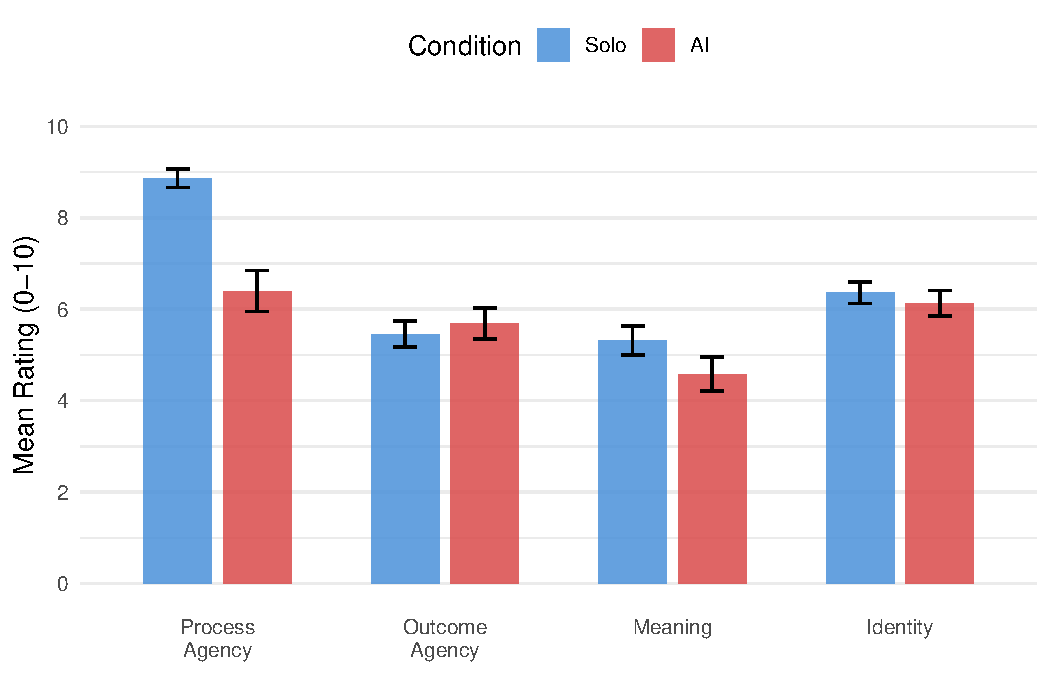
\includegraphics[width=\linewidth]{../output/figures/fig_composites.pdf}
  \caption{Survey composites by condition. Error bars represent $\pm$1 SE.}
  \label{fig:composites}
\end{figure}

\begin{figure}[t]
  \centering
  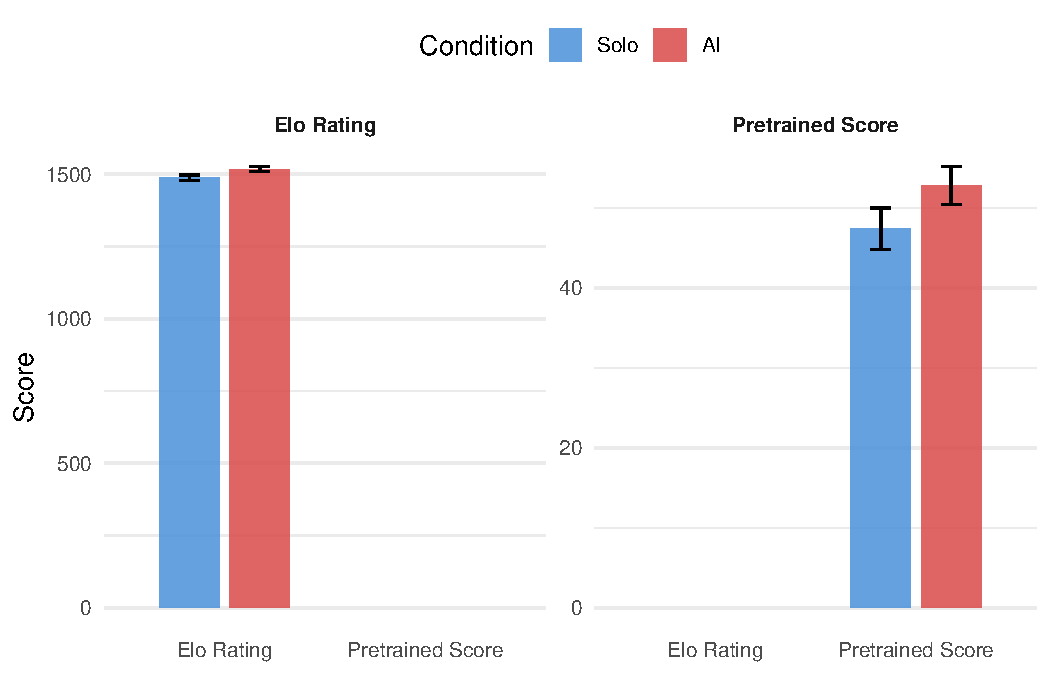
\includegraphics[width=\linewidth]{../output/figures/fig_quality.pdf}
  \caption{Caption quality by condition. Error bars represent $\pm$1 SE.}
  \label{fig:quality}
\end{figure}

\end{document}
